\section{Toward an Embodied Learning Environment for Teaching
Geometry}\label{toward-an-embodied-learning-environment-for-teaching-geometry}

\textbf{Andreas Papasalouros¹ and Antonios Kontogiannis²}

¹Associate Professor, Department of Mathematics, University of the
Aegean ²PhD Candidate, Department of Mathematics, University of the
Aegean

\subsection{Abstract}\label{abstract}

This chapter presents a technology-enhanced environment designed to
support embodied learning activities in geometry by leveraging recent
advances in computer vision and artificial intelligence. The design of
the environment is grounded in theories of embodied and enactive
cognition, which emphasize that learning emerges through active bodily
engagement, movement, and interaction with the physical environment.
Building upon these theoretical foundations, the chapter introduces a
collaborative smart classroom platform that enables students to
construct and explore geometric concepts through coordinated full-body
activity.

Within the proposed environment, students' positions are continuously
tracked in real time and mapped onto a shared geometric representation
displayed on a classroom screen. Each participant embodies a geometric
object---typically a point---whose movement in the physical space
produces corresponding transformations within an idealized geometric
workspace. Unlike conventional geometry instruction, where students
primarily observe or manipulate virtual representations, the proposed
approach enables learners to collaboratively construct and transform
geometric configurations through coordinated movement, communication,
and interaction. The teacher orchestrates each activity by defining
geometric objects and constraints, while students collectively
manipulate these objects through their physical actions.

The environment has been designed to require only inexpensive and widely
available classroom equipment, consisting of a standard camera, a
computer, and a projector or large display. Real-time interaction is
supported through deep-learning-based multi-object detection and
tracking, allowing accurate localization and persistent identification
of multiple participants throughout the learning activity. The software
has been implemented as a reusable framework that can be readily adapted
to a variety of geometry applications and, more generally, to other
educational domains where tracking learners' positions and interactions
can support meaningful learning experiences.

A formative pilot evaluation was conducted during a two-hour session
involving three students aged 10--14. Four collaborative geometry
activities were implemented, including navigating predefined geometric
locations, constructing symmetric points, and collaboratively forming
equilateral and right triangles. The results demonstrated that the
proposed environment provides sufficient technical accuracy and
responsiveness to support embodied geometry activities. Students
successfully completed all tasks, remained actively engaged throughout
the session, and described the experience as more interesting and less
monotonous than conventional classroom instruction.

The pilot study also identified several directions for further
development. These include reducing positional jitter caused by natural
body movements, improving participant re-identification following
temporary occlusions, providing richer instructional scaffolding for
complex collaborative tasks, and incorporating immediate visual feedback
to support successful task completion. Future work will focus on
expanding the range of curriculum-aligned activities, conducting
larger-scale classroom studies, and investigating additional interaction
modalities, such as gesture recognition. Beyond this specific
application, the proposed environment illustrates how contemporary
computer vision technologies can facilitate the implementation of
embodied learning in ordinary classrooms through a low-cost, reusable,
and easily deployable platform.

\textbf{Keywords:} embodied learning; geometry education; smart
classroom; collaborative learning; computer vision; mathematics
education.

\subsection{2. Introduction}\label{introduction}

Theories of embodied and enactive cognition (Varela, Thompson, and Rosch
1991; Tsakiri 2010) extend the constructivist view of learning by
arguing that knowledge is not acquired solely through observation or
information transfer but emerges through learners' active engagement
with their environment. These perspectives emphasize that cognition is
fundamentally grounded in bodily action and situated interaction,
highlighting the importance of movement, gesture, and physical
participation in authentic learning contexts.

Within mathematics education, embodied cognition has received
considerable attention over the past two decades. A growing body of
research argues that mathematical thinking is inherently embodied
(Alibali and Nathan 2012; Papert 1991), with even highly abstract
mathematical concepts being rooted in learners' sensorimotor experiences
and their interactions with the physical world (Lakoff and Núñez 2000).
Consequently, learning mathematics is increasingly viewed not merely as
the manipulation of abstract symbolic representations but as a process
that is closely connected to perception, action, and spatial experience.

These theoretical developments have stimulated substantial research on
embodied learning within STEM education (Junus et al. 2024). In
parallel, systematic design principles have been proposed for developing
embodied learning activities, particularly in mathematics education,
where physical interaction is intentionally integrated with conceptual
understanding (Abrahamson et al. 2020; Smith and Walkington 2019).

From the perspective of embodied cognition, learning environments should
encourage learners to actively participate in the systems they seek to
understand rather than observe them from a detached standpoint. This
principle has motivated the development of participatory simulations and
role-playing learning environments (Colella 2000; Resnick and Wilensky
1998), in which students become integral components of the phenomena or
mathematical structures under investigation. Such environments are
frequently implemented within smart classrooms (Lui and Slotta 2014;
Tissenbaum and Slotta 2014), where sensing technologies, networked
devices, and large shared displays enable students to interact with one
another while jointly constructing knowledge through physical activity.

A defining characteristic of these environments is that learners engage
through movement within a shared physical space rather than remaining
seated in front of individual computers. At the same time, collaboration
emerges naturally through face-to-face communication, coordinated bodily
actions, and shared interaction with digital representations. This
combination of physical participation, social interaction, and
technological support provides a promising foundation for designing
learning experiences that bridge abstract mathematical concepts with
students' embodied experiences.

Building upon these principles, this chapter presents an embodied
learning environment specifically designed to support geometry education
through collaborative full-body interaction. Unlike existing systems
that often rely on specialized sensing equipment, the proposed
environment employs only a conventional camera together with recent
computer vision and artificial intelligence techniques to provide
accurate real-time tracking of multiple students. The system has been
designed as a reusable software framework capable of supporting a wide
range of collaborative geometry activities while remaining inexpensive,
easily deployable, and suitable for ordinary classroom settings.

\subsection{3. Embodied Learning, Tracking Technologies, and Related
Learning
Environments}\label{embodied-learning-tracking-technologies-and-related-learning-environments}

Recent advances in digital technologies have significantly expanded the
possibilities for implementing embodied learning across a wide range of
educational settings. Contemporary embodied learning environments
increasingly integrate technologies such as virtual and augmented
reality, motion capture, depth sensors, computer vision, and artificial
intelligence to establish a direct relationship between learners'
physical actions and digital representations (Abrahamson, Ryokai, and
Dimmel 2023). Within these environments, students' movements and
gestures are continuously monitored and interpreted in real time,
allowing the system to provide immediate visual or multimodal feedback
that strengthens the connection between bodily action and conceptual
understanding.

In mathematics education, these technologies allow physical movement to
acquire explicit mathematical meaning. Rather than functioning merely as
interaction techniques, gestures and bodily movements become
representations of mathematical objects and relationships, enabling
learners to experience abstract concepts through sensorimotor activity
(Smith and Walkington 2019). This close coupling between action and
representation has been shown to facilitate conceptual understanding
while increasing learner engagement.

A considerable number of embodied learning environments have been
developed to support mathematics and science education. One of the
earliest examples is \textbf{SMALLab Learning} (Birchfield and
Megowan-Romanowicz 2009), which combines motion-tracking technologies
with large-scale immersive visualizations, allowing students to explore
mathematical and scientific concepts through full-body interaction. The
\textbf{Mathematical Imagery Trainer (MIT)} (Abrahamson and Trninic
2015) enables learners to manipulate mathematical representations
through carefully designed gestures, providing immediate visual feedback
that supports the gradual construction of mathematical meaning.

More recent environments have incorporated mixed reality and computer
vision technologies. \textbf{Mathland} (Khan, Trujano, and Maes 2018)
employs Microsoft HoloLens to support embodied interaction with
mathematical concepts in immersive mixed-reality settings, while
\textbf{Leap Motion Math} (Na and Sung 2025) enables students to
manipulate geometric objects through natural hand and finger movements
using Leap Motion sensors in combination with augmented reality
techniques.

Beyond commercially available platforms such as Kinect and Wii,
researchers have also developed specialized embodied learning systems
tailored to particular educational objectives. For example,
\textbf{Polymichanon} (Kynigos, Smyrnaiou, and Roussou 2010) supports
precise motion tracking and the mapping of learners' movements onto
mathematical representations. A consistent finding across these studies
is that guided bodily interaction can promote deeper conceptual
understanding of mathematical relationships (Abrahamson, Ryokai, and
Dimmel 2023), improve spatial reasoning through immersive environments
(Kynigos, Smyrnaiou, and Roussou 2010), and enhance participation and
confidence among students with special educational needs (Kourakli et
al. 2017).

Overall, the evaluation of these embodied learning environments suggests
that meaningful bodily interaction can enhance conceptual understanding,
increase learner motivation, and promote collaborative forms of
learning. Nevertheless, many existing systems depend on specialized
hardware, including depth cameras, wearable sensors, dedicated
controllers, or immersive visualization equipment, limiting their
scalability and adoption in everyday classroom settings.

The environment proposed in this study follows a different design
philosophy. Instead of relying on specialized sensing technologies, it
uses a single conventional camera together with state-of-the-art
deep-learning-based computer vision techniques to detect, identify, and
track multiple students in real time. This substantially reduces
equipment requirements while preserving the core affordances necessary
to support collaborative embodied learning activities. Consequently, the
proposed environment offers a practical and cost-effective solution that
can be deployed in ordinary school classrooms without requiring
specialized infrastructure.

\subsection{4. STROBE: A new environment for Embodied Learning in
Mathematics}\label{strobe-a-new-environment-for-embodied-learning-in-mathematics}

The environment presented in this chapter has been designed to support
collaborative embodied learning activities in geometry through the
real-time tracking of students' positions within the physical classroom.
The primary objective is not merely to provide a novel interaction
technology, but to establish a research platform for designing,
implementing, and evaluating embodied learning activities that
\textbf{promote conceptual understanding} through physical participation
and collaboration.

Geometry provides an especially suitable context for this approach.
Although students are generally able to recognize common geometric
figures, numerous studies have shown that they often experience
difficulties in understanding their properties and the relationships
among geometric objects (Sarama and Clements 2019). Embodied learning
offers an alternative perspective by allowing abstract geometric
concepts to emerge through learners' bodily actions rather than through
symbolic manipulation alone.

Within the proposed environment, each participant embodies a geometric
object, typically a point within a geometric construction. Students move
freely inside the physical classroom, while their positions are
continuously detected and transformed into corresponding coordinates
within an idealized geometric workspace. These representations are
displayed on a shared classroom screen, allowing all participants to
observe both their own embodied representation and those of their
classmates in real time.

Following the principles of participatory simulations and educational
role-playing (Colella 2000; Resnick and Wilensky 1998), students become
active components of the mathematical construction itself rather than
external observers. As participants move, the geometric objects they
represent move accordingly, together with all dependent objects within
the construction, in a manner similar to a dynamic geometry environment.
Consequently, students experience geometric relationships not only
through visual observation but also through direct physical interaction.

The teacher orchestrates each activity by defining the geometric objects
and constraints that frame students' actions. For example, the teacher
may create a line of symmetry, specify the vertices of a geometric
figure, or establish other construction rules that students must satisfy
collaboratively through coordinated movement. In this way, the
environment combines the flexibility of dynamic geometry software with
the pedagogical affordances of embodied participation.

The design of the environment aims to strengthen students' sense of
presence and encourage collaboration throughout the learning process.
Whereas conventional mathematics instruction often positions learners as
detached observers manipulating abstract representations, embodied
learning places students at the centre of the activity, allowing them to
experience mathematical ideas from a first-person perspective
(Mikropoulos 2006; Smith 2018). By identifying themselves with the
geometric objects they represent---or, in Papert's (1991) terms, by
\emph{becoming} those objects---students actively participate in the
formation and transformation of geometric constructions while
simultaneously observing both the shared digital representation and the
physical actions of their peers.

This embodied participation supports communication, \textbf{joint
problem solving}, and \textbf{the negotiation of meaning among group
members}. Students coordinate their movements through face-to-face
interaction while collectively pursuing a common geometric objective.
Such collaboration not only promotes communication but also distributes
the cognitive demands of complex tasks, allowing learners to focus on
different aspects of the construction, thereby facilitating conceptual
understanding (Smith and Walkington 2019).

Accordingly, the proposed environment should be viewed not simply as a
motion-tracking system, but as an embodied collaborative learning
platform in which physical movement, social interaction, and dynamic
geometric representations are integrated into a unified learning
experience.

\subsection{5. Pedagogical and Technical
Affordances}\label{pedagogical-and-technical-affordances}

The proposed environment has been designed to provide a set of
affordances that support collaborative embodied learning activities
while maintaining the simplicity required for deployment in ordinary
classroom settings. These affordances arise from the integration of
computer vision technologies with pedagogically informed interaction
design.

\subsubsection{5.1 Real-Time Multi-Participant
Tracking}\label{real-time-multi-participant-tracking}

A fundamental affordance of the environment is the ability to accurately
determine the positions of multiple students simultaneously and in real
time. Continuous position tracking enables learners to interact
naturally within the physical classroom while receiving immediate visual
feedback through the shared geometric representation. This close
temporal coupling between movement and visual representation strengthens
the embodied connection between physical action and mathematical
meaning.

\subsubsection{5.2 Persistent Participant
Identification}\label{persistent-participant-identification}

Beyond position tracking, the environment maintains the identity of each
participant throughout the learning activity. Each student is
continuously identified using visual appearance features, allowing the
system to preserve the correspondence between a learner and the
geometric object that he or she represents, even after temporary
disappearance or re-entry into the interaction space. Persistent
identification is essential for collaborative activities in which
students remain responsible for specific geometric entities during the
construction process.

\subsubsection{5.3 Shared Visual
Workspace}\label{shared-visual-workspace}

The environment provides a common visual representation of the activity
through a projector or large classroom display. Students observe both
their own positions and those of their classmates within the same
geometric workspace, together with any additional information required
by the activity. This shared representation establishes a common frame
of reference that supports communication, coordination, and
collaborative problem solving.

\subsubsection{5.4 Teacher-Orchestrated Geometric
Constraints}\label{teacher-orchestrated-geometric-constraints}

The teacher can define geometric objects and construction constraints
that shape the collaborative activity. Examples include symmetry axes,
line segments, circles, predefined vertices, or other geometric
structures that students must collectively manipulate through their
movements. Rather than controlling the activity directly, the teacher
orchestrates the learning process by designing the mathematical
\textbf{situation} within which students interact.

\subsubsection{5.5 Low-Cost and Easily Deployable
Infrastructure}\label{low-cost-and-easily-deployable-infrastructure}

A central design objective of the proposed environment is
\textbf{accessibility}. The system requires only equipment that is
already available in most schools---a conventional camera, a computer,
and a projector or large display. Consequently, embodied learning
activities can be implemented without specialized hardware such as depth
sensors, wearable devices, or immersive virtual reality systems.

\subsubsection{5.6 Reusability Beyond
Geometry}\label{reusability-beyond-geometry}

Although the present implementation focuses on geometry education, the
underlying software framework has been designed to support a
considerably broader range of educational applications. Any learning
activity that benefits from monitoring the positions, movements, or
interactions of multiple participants can build upon the same
technological infrastructure. Consequently, the proposed framework
provides a reusable foundation for the development of embodied learning
environments across different subject domains.

\subsection{6. Implementation}\label{implementation}

The implementation of the proposed environment was driven by the
technical requirements derived from the pedagogical objectives presented
in the previous sections. In particular, the system had to support the
accurate localization of multiple students, maintain their identities
throughout the interaction, and provide real-time visual feedback with
sufficiently low latency to preserve the embodied nature of the learning
experience.

To satisfy these requirements, the environment employs a
deep-learning-based multi-object tracking pipeline. Multi-object
tracking (MOT) has recently attracted considerable attention in
application domains such as intelligent transportation, sports
analytics, robotics, and precision agriculture (Xu 2023). The same
technological advances provide an effective foundation for educational
environments in which multiple learners interact simultaneously within a
shared physical space.

The tracking pipeline consists of two complementary stages: object
detection and object tracking. During the detection stage, the system
identifies all people visible within the camera's field of view and
estimates their locations in each video frame. Detection is performed
using the YOLO object detection framework (Jocher, Chaurasia, and Qiu
2023), selected for its high detection accuracy and real-time
performance.

The second stage associates the detected individuals across consecutive
frames in order to preserve their identities throughout the learning
activity. Following an extensive evaluation of several contemporary
multi-object tracking algorithms, a DeepSORT-based implementation
(Wojke, Bewley, and Paulus 2017) was selected as the most suitable
solution for the requirements of the proposed environment. This approach
combines motion prediction with appearance-based re-identification,
allowing participants to retain consistent identities even during
temporary interruptions in visual tracking.

The complete tracking pipeline operates continuously in real time. For
every incoming video frame, the system detects the participants, updates
their identities, estimates their positions within the interaction
space, and transmits the resulting coordinates to the educational
application. The application subsequently updates the shared geometric
workspace, allowing students to observe the immediate consequences of
their physical movements on the projected geometric construction.

The software has been developed as an open-source, reusable framework
rather than as a single-purpose educational application. This design
enables developers and researchers to implement different embodied
learning scenarios while reusing the same tracking infrastructure.
Although the present work focuses on geometry education, the framework
is intended to support a much broader range of educational applications
involving collaborative embodied interaction.

The software developed for this work is publicly available as
open-source software through the STROBE project on GitHub. The framework
has been designed to facilitate future extensions, including support for
additional interaction techniques, alternative tracking algorithms, and
new educational activities, while preserving a common software
architecture for embodied learning applications.

\subsection{7. Pilot Evaluation}\label{pilot-evaluation}

\subsubsection{7.1 Method}\label{method}

The proposed environment was evaluated through a formative pilot study
following the principles of Learner-Centered Design (LCD) (Quintana et
al. 2006). Rather than attempting to measure learning outcomes, the
evaluation focused on examining the usability of the environment, the
technical reliability of the tracking system, and its ability to support
the intended embodied learning activities under realistic conditions.

The pilot study pursued four main objectives:

\begin{itemize}
\tightlist
\item
  to evaluate the technical reliability of the multi-student detection
  and tracking mechanism;
\item
  to assess the usability and functionality of the environment during
  collaborative geometry activities;
\item
  to investigate students' cognitive and collaborative engagement
  throughout the activities; and
\item
  to identify design improvements for increasing the pedagogical
  effectiveness of the environment.
\end{itemize}

The evaluation was conducted during a two-hour session in May 2025 with
three students aged 10, 12, and 14 years. Although the sample size was
intentionally small, the purpose of the study was formative rather than
summative, aiming to identify technical limitations and usability issues
before conducting larger classroom evaluations.

The students completed four collaborative geometry activities designed
according to the principles for embodied mathematics learning proposed
by Smith and Walkington (Smith and Walkington 2019).

\textbf{Activity 1 -- Navigating the Vertices of a Square}

Each student individually moved successively among four predefined
locations corresponding to the vertices of a square. The positions were
physically marked within the interaction space rather than displayed on
the projected geometric representation. Students remained stationary at
each location until instructed by the facilitator to move to the next
vertex.

\textbf{Activity 2 -- Constructing Symmetric Points}

A vertical line representing an axis of symmetry was displayed on the
shared screen. One student selected an arbitrary position within the
interaction area, while a second student attempted to position
themselves at the corresponding symmetric point with respect to the
displayed axis.

\textbf{Activity 3 -- Constructing an Equilateral Triangle}

Two students first established the endpoints of a line segment by
remaining stationary. The third student then moved until the three
embodied points formed an equilateral triangle. The activity was
repeated several times while students alternated roles.

\textbf{Activity 4 -- Constructing a Right Triangle}

The three students collaboratively formed a right triangle starting from
arbitrary positions within the interaction space. The youngest
participant was assigned the role of the vertex containing the right
angle. As in the previous activity, students exchanged roles across
successive trials. ::: \{\#fig:geometry-environment\}

\begin{figure}
\centering
\pandocbounded{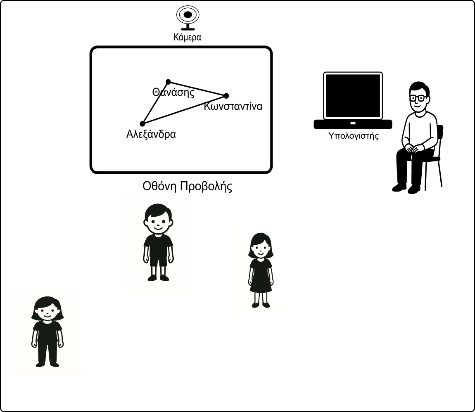
\includegraphics[keepaspectratio]{images/image1.png}}
\caption{Visual representation of the collaborative learning environment
for Geometry}
\end{figure}

\begin{figure}
\centering
\pandocbounded{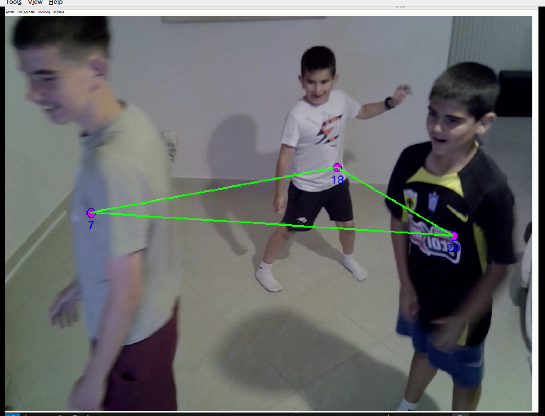
\includegraphics[keepaspectratio]{images/image2.png}}
\caption{Screenshot of the implementation of Activity 3}
\end{figure}

Visual representation of the collaborative learning environment for
Geometry (left) and screenshot of the implementation of Activity 3
(right).

:::

\subsubsection{7.2 Experimental Setting and Data
Collection}\label{experimental-setting-and-data-collection}

The activities were facilitated by one of the authors, who provided the
initial instructions and coordinated the progression of the tasks.
Students were explicitly encouraged to communicate continuously with one
another throughout the activities in order to support collaborative
problem solving.

The evaluation was conducted in a 4 × 4 m indoor space. A single camera
was mounted at a height of approximately 2.1 m above the floor,
providing an oblique view of the interaction area. A geometric
correction was applied to compensate for the camera perspective before
mapping participants' positions onto the shared geometric workspace. The
visual representation was projected on a 65-inch display.

Three complementary sources of data were collected during the
evaluation:

\begin{enumerate}
\def\labelenumi{\arabic{enumi}.}
\item
  \textbf{System logs}, containing the real-time coordinates of all
  participants throughout each activity.
\item
  \textbf{Video recordings}, used to analyse students' movements,
  collaboration patterns, engagement, communication, and interaction
  with the environment. Written parental consent was obtained for both
  data collection and the publication of photographs showing the
  participating students.
\item
  \textbf{Semi-structured interviews}, conducted immediately after the
  session, during which students reflected on the usability of the
  environment, their understanding of the mathematical concepts
  involved, and their overall learning experience.
\end{enumerate}

The collected data were analysed qualitatively. Given that the
environment is still under active development, the primary objective of
the analysis was not to produce generalisable findings but rather to
identify technical limitations, usability issues, and pedagogical design
improvements that will inform future iterations of the system.

\subsection{8. Results and Discussion}\label{results-and-discussion}

\subsubsection{8.1 Technical Performance}\label{technical-performance}

The first objective of the pilot evaluation was to examine the technical
reliability of the proposed environment. In particular, we evaluated the
accuracy of participant localization and the consistency of multi-object
identification throughout the collaborative activities.

Overall, the system demonstrated \textbf{satisfactory performance} for
the intended educational scenarios. Position estimation proved
sufficiently accurate to support all four geometry activities, while
participant identities remained stable throughout the interaction
whenever students remained within the camera's field of view. The
average end-to-end system latency---including detection, tracking, and
visualization---was approximately 85 ms, providing a sufficiently
responsive interaction to preserve the \textbf{embodied character} of
the activities. Performance measurements were obtained using a
workstation equipped with an AMD Ryzen 7 3800X processor, 16 GB RAM, and
an NVIDIA GeForce GTX 1660 graphics card with 6 GB of dedicated memory.

These results suggest that recent deep-learning-based tracking
technologies can provide the responsiveness and reliability required for
collaborative embodied learning activities without relying on
specialized sensing equipment.

\subsubsection{8.2 Students' Participation and Learning
Experience}\label{students-participation-and-learning-experience}

All participants successfully completed the four collaborative geometry
activities. Throughout the evaluation, students remained actively
engaged and collaborated effectively in achieving the objectives of each
task.

The second activity, involving the construction of symmetric points, was
completed easily by all participants, indicating that the embodied
representation of geometric symmetry was readily understood. The third
activity, which required the collaborative construction of an
equilateral triangle, proved more challenging but was completed
successfully after a limited number of attempts.

The fourth activity -- constructing a right triangle -- presented the
greatest level of difficulty. Students required substantially more time,
approximately six minutes, and several successive attempts before
successfully completing the task. Observation of the activity suggested
that the difficulty arose from two complementary factors. First,
students needed to recognize and maintain the appropriate geometric
relationships among the three vertices while continuously adjusting
their own positions. Second, they were required to coordinate their
movements collaboratively, making simultaneous decisions about both
individual positioning and group strategy.

Communication during this activity was particularly rich. Students
continuously negotiated possible solutions through verbal discussion,
gestures, and even physical guidance, with the oldest participant
assisting the younger students in achieving the desired configuration.
These observations illustrate the collaborative character of the
environment and demonstrate how embodied interaction naturally promotes
communication and joint problem solving.

The post-activity interviews further confirmed students' positive
perceptions of the learning experience. One participant summarized the
experience by stating:

\begin{quote}
\emph{``It was enjoyable. It was less boring than a normal lesson. I'm
not sure whether we learned more, but it was definitely more
interesting.''}
\end{quote}

Although informal, this comment reflects the increased engagement
observed throughout the evaluation. Furthermore, students were able to
recall the objectives of each activity and explain the mathematical
concepts involved, even when their mathematical terminology was not
always fully precise.

\subsubsection{8.3 Observed Limitations}\label{observed-limitations}

The pilot study also revealed several technical and pedagogical
limitations that will guide future development of the environment.

Although participant localization was generally accurate, natural body
movements -- particularly arm movements -- occasionally caused small
fluctuations in the detected position. This issue became most evident
during the first activity, where students were required to remain
stationary at predefined locations. The observed positional jitter
resulted primarily from changes in the body outline detected by the YOLO
object detector, which is inherently sensitive to variations in body
posture and gesture.

Potential solutions include replacing the current detection and tracking
pipeline with approaches such as FairMOT or incorporating an additional
camera to improve localization accuracy. While the latter option would
likely enhance robustness, it would also increase both hardware
complexity and deployment cost, reducing one of the principal advantages
of the proposed environment.

A second limitation involved participant re-identification following
temporary occlusions. In a small number of cases, the system failed to
recover a participant's original identity after one student temporarily
obscured another. Although this issue did not interfere with the
activities performed during the pilot study, it highlighted the
importance of robust identity preservation in collaborative embodied
environments. Following the completion of the pilot evaluation,
adjustments to the tracking parameters substantially improved this
behaviour.

\subsubsection{8.4 Implications for Future
Design}\label{implications-for-future-design}

Beyond the technical observations, the pilot study provided valuable
insights into the pedagogical design of embodied learning activities.

One important finding concerned the need for immediate visual feedback.
During the evaluation, participants relied primarily on verbal guidance
from the facilitator to determine whether an activity had been completed
successfully. Future versions of the environment will therefore
incorporate automatic visual feedback, similar to that employed in the
Mathematics Imagery Trainer, enabling students to receive continuous
information about their progress without external intervention.

The evaluation also highlighted the importance of instructional
scaffolding during complex collaborative activities. The right-triangle
construction required students not only to control their own movements
but also to coordinate their actions with those of their peers while
reasoning about geometric relationships. General verbal instructions
proved insufficient for supporting this process. Future activities will
therefore incorporate more explicit collaboration scripts,
micro-scenarios, and problem-solving strategies to guide learners
through increasingly demanding collaborative tasks.

Finally, it should be acknowledged that the positive reactions reported
by the participants may partly reflect the novelty of the experience
rather than the intrinsic educational effectiveness of the environment.
Consequently, the present findings should be interpreted as formative
rather than conclusive. Larger and longer-term classroom studies will be
required to investigate the sustained educational impact of the proposed
environment under authentic teaching conditions.

\subsection{9. Conclusions and Future
Work}\label{conclusions-and-future-work}

This chapter presented the design, implementation, and formative
evaluation of a collaborative embodied learning environment for geometry
that combines computer vision, artificial intelligence, and embodied
learning principles. The proposed environment enables students to engage
with geometric concepts through coordinated physical movement,
collaboration, and real-time interaction within a shared digital
workspace.

Unlike many existing embodied learning environments, the proposed system
has been designed to operate using only widely available classroom
equipment, including a conventional camera, a computer, and a projector
or large display. By combining recent advances in deep-learning-based
multi-object tracking with a reusable software architecture, the
environment provides a practical and scalable platform that can support
embodied learning activities without requiring specialized sensing
technologies or immersive installations.

The formative pilot evaluation demonstrated that the environment is
technically capable of supporting collaborative geometry activities
involving multiple participants. Students successfully completed all
four learning activities, remained actively engaged throughout the
session, and reported positive perceptions of the overall learning
experience. At the same time, the evaluation identified several
technical and pedagogical challenges that will guide future development,
including improving positional stability, strengthening participant
re-identification following temporary occlusions, providing richer
instructional scaffolding, and incorporating more informative real-time
visual feedback.

Although this was only a small formative study, our findings suggest
that deep-learning-based tracking can provide a workable foundation for
embodied learning in real classrooms. Crucially, because our system
relies on a standard camera rather than depth sensors or wearables, it
demonstrates a practical path toward making embodied geometry activities
accessible to ordinary schools.

Our future agenda comprises three strands. First, we will develop
additional curriculum-aligned activities, focusing particularly on the
concept of angle and geometric transformations. Second, we intend to
replace positional tracking with full-body pose estimation (e.g.,
MediaPipe), which would allow us to capture students' gestures and
posture as additional data streams. Third, we have initiated discussions
with local schools to plan a larger, longitudinal study that will assess
retention and transfer of geometric understanding. While we currently
target geometry, we view the underlying software as a general-purpose
orchestration tool---one that we believe is equally applicable to any
domain where group coordination and spatial decision-making are
pedagogically relevant.

\phantomsection\label{refs}
\begin{CSLReferences}{1}{0}
\bibitem[\citeproctext]{ref-AbrahamsonNathan2020}
Abrahamson, Dor, Mitchell J. Nathan, Caro Williams-Pierce, Candace
Walkington, Erin R. Ottmar, Hortensia Soto, and Martha W. Alibali. 2020.
{``The Future of Embodied Design for Mathematics Teaching and
Learning.''} \emph{Frontiers in Education} 5 (147).
\url{https://doi.org/10.3389/feduc.2020.00147}.

\bibitem[\citeproctext]{ref-AbrahamsonRyokaiDimmel2023}
Abrahamson, Dor, Kimiko Ryokai, and Justin Dimmel. 2023. {``Learning
Mathematics with Digital Resources: Reclaiming the Cognitive Role of
Physical Movement.''} In \emph{Handbook of Digital Resources in
Mathematics Education}, edited by Birgit Pepin, Ghislaine Gueudet, and
Jeffrey Choppin, 1--37. Cham: Springer.
\url{https://doi.org/10.1007/978-3-030-95060-6_22-1}.

\bibitem[\citeproctext]{ref-AbrahamsonTrninic2015}
Abrahamson, Dor, and Dragan Trninic. 2015. {``Bringing Forth
Mathematical Concepts: Signifying Sensorimotor Enactment in Fields of
Promoted Action.''} \emph{ZDM Mathematics Education} 47 (2): 295--306.
\url{https://doi.org/10.1007/s11858-014-0620-0}.

\bibitem[\citeproctext]{ref-AlibaliNathan2012}
Alibali, Martha W., and Mitchell J. Nathan. 2012. {``Embodiment in
Mathematics Teaching and Learning: Evidence from Learners' and Teachers'
Gestures.''} \emph{Journal of the Learning Sciences} 21 (2): 247--86.
\url{https://doi.org/10.1080/10508406.2011.611446}.

\bibitem[\citeproctext]{ref-BirchfieldMegowanRomanowicz2009}
Birchfield, David, and Colleen Megowan-Romanowicz. 2009. {``Earth
Science Learning in SMALLab: A Design Experiment for Mixed Reality.''}
\emph{International Journal of Computer-Supported Collaborative
Learning} 4 (4): 403--21.
\url{https://doi.org/10.1007/s11412-009-9074-8}.

\bibitem[\citeproctext]{ref-Colella2000}
Colella, Vanessa. 2000. {``Participatory Simulations: Building
Collaborative Understanding Through Immersive Dynamic Modeling.''}
\emph{Journal of the Learning Sciences} 9 (4): 471--500.
\url{https://doi.org/10.1207/S15327809JLS0904_4}.

\bibitem[\citeproctext]{ref-JocherUltralytics2023}
Jocher, Glenn, Ayush Chaurasia, and Jing Qiu. 2023. {``Ultralytics
YOLOv8.''} \url{https://github.com/ultralytics/ultralytics}.

\bibitem[\citeproctext]{ref-Junus2024}
Junus, Fadhla B., Junior Anthony Bennett, Theresa Green, Jason W.
Morphew, and Ruth Wertz. 2024. {``Visuospatial and Embodied Cognition in
STEM Education: A Systematic Literature Review.''} In \emph{2024 ASEE
Annual Conference \& Exposition}. Portland, Oregon: ASEE Conferences.
\url{https://doi.org/10.18260/1-2--48261}.

\bibitem[\citeproctext]{ref-KhanTrujanoMaes2018}
Khan, Mina, Fernando Trujano, and Pattie Maes. 2018. {``Mathland:
Constructionist Mathematical Learning in the Real World Using Immersive
Mixed Reality.''} In \emph{Immersive Learning Research Network}, edited
by Dennis Beck, Colin Allison, Leonel Morgado, Johanna Pirker, Anasol
Peña-Rios, Todd Ogle, Jonathon Richter, and Christian Gütl, 840:133--47.
Communications in Computer and Information Science. Cham: Springer.
\url{https://doi.org/10.1007/978-3-319-93596-6_9}.

\bibitem[\citeproctext]{ref-Kourakli2017}
Kourakli, Maria, Ioannis Altanis, Symeon Retalis, Michail Boloudakis,
Dimitrios Zbainos, and Katerina Antonopoulou. 2017. {``Towards the
Improvement of the Cognitive, Motoric and Academic Skills of Students
with Special Educational Needs Using Kinect Learning Games.''}
\emph{International Journal of Child-Computer Interaction} 11: 28--39.
\url{https://doi.org/10.1016/j.ijcci.2016.10.009}.

\bibitem[\citeproctext]{ref-KynigosSmyrnaiouRoussou2010}
Kynigos, Chronis, Zacharoula Smyrnaiou, and Maria Roussou. 2010.
{``Exploring Rules and Underlying Concepts While Engaged with
Collaborative Full-Body Games.''} In \emph{Proceedings of the 9th
International Conference on Interaction Design and Children (IDC '10)},
222--25. Barcelona, Spain: ACM.
\url{https://doi.org/10.1145/1810543.1810576}.

\bibitem[\citeproctext]{ref-LakoffNunez2000}
Lakoff, George, and Rafael E. Núñez. 2000. \emph{Where Mathematics Comes
from: How the Embodied Mind Brings Mathematics into Being}. New York,
NY: Basic Books.

\bibitem[\citeproctext]{ref-LuiSlotta2014}
Lui, Michelle, and James D. Slotta. 2014. {``Immersive Simulations for
Smart Classrooms: Exploring Evolutionary Concepts in Secondary
Science.''} \emph{Technology, Pedagogy and Education} 23 (1): 57--80.
\url{https://doi.org/10.1080/1475939X.2013.838452}.

\bibitem[\citeproctext]{ref-Mikropoulos2006}
Mikropoulos, Tassos A. 2006. {``Presence: A Unique Characteristic in
Educational Virtual Environments.''} \emph{Virtual Reality} 10 (3--4):
197--206. \url{https://doi.org/10.1007/s10055-006-0039-1}.

\bibitem[\citeproctext]{ref-NaSung2025}
Na, Hunhui, and Hanall Sung. 2025. {``Learn Math Through Motion: A
Technology-Enhanced Embodied Approach with Augmented Reality for
Geometry Learning in k-12 Classrooms.''} \emph{Interactive Learning
Environments} 33 (6): 3744--57.
\url{https://doi.org/10.1080/10494820.2025.2450663}.

\bibitem[\citeproctext]{ref-Papert1991}
Papert, Seymour. 1991. \emph{Noitikes Thyelles: Paidia, Ilektronikoi
Ypologistes Kai Dynamikes Idees}. Athens: Odysseas.

\bibitem[\citeproctext]{ref-QuintanaShinNorrisSoloway2006}
Quintana, Chris, Namsoo Shin, Cathleen Norris, and Elliot Soloway. 2006.
{``Learner-Centered Design: Reflections on the Past and Directions for
the Future.''} In \emph{The Cambridge Handbook of the Learning
Sciences}, edited by R. Keith Sawyer, 119--34. Cambridge: Cambridge
University Press. \url{https://doi.org/10.1017/CBO9780511816833.009}.

\bibitem[\citeproctext]{ref-Resnick1998}
Resnick, Mitchel, and Uri Wilensky. 1998. {``Diving into Complexity:
Developing Probabilistic Decentralized Thinking Through Role-Playing
Activities.''} \emph{Journal of the Learning Sciences} 7 (2): 153--72.
\url{https://doi.org/10.1207/s15327809jls0702_1}.

\bibitem[\citeproctext]{ref-SaramaClements2019}
Sarama, Julie, and Douglas H. Clements. 2019. {``Learning Trajectories
in Early Mathematics Education.''} In \emph{Researching and Using
Progressions (Trajectories) in Mathematics Education}, edited by Dianne
Siemon, Tasos Barkatsas, and Rebecca Seah, 32--55. Sense Publishers.
\url{https://doi.org/10.1163/9789004396449_002}.

\bibitem[\citeproctext]{ref-Smith2018}
Smith, Carmen Petrick. 2018. {``Body-Based Activities in Secondary
Geometry: An Analysis of Learning and Viewpoint.''} \emph{School Science
and Mathematics} 118 (5): 179--89.
\url{https://doi.org/10.1111/ssm.12279}.

\bibitem[\citeproctext]{ref-Smith2019}
Smith, Carmen Petrick, and Candace Walkington. 2019. {``Four Principles
for Designing Embodied Mathematics Activities.''} \emph{Australian
Mathematics Education Journal} 1 (4): 16--20.

\bibitem[\citeproctext]{ref-Tissenbaum2014}
Tissenbaum, Mike, and James D. Slotta. 2014. {``Developing an
Orchestrational Framework for Collective Inquiry in Smart Classrooms:
SAIL Smart Space (S3).''} In \emph{Learning and Becoming in Practice:
The International Conference of the Learning Sciences (ICLS) 2014},
edited by Joseph L. Polman, Eleni A. Kyza, D. Kevin O'Neill, Iris Tabak,
William R. Penuel, A. Susan Jurow, Kevin O'Connor, Tiffany Lee, and
Laura D'Amico, 2:831--38. Boulder, CO: International Society of the
Learning Sciences.

\bibitem[\citeproctext]{ref-Tsakiri2010}
Tsakiri, Amalia. 2010. {``I Syneidisi Os Anadyomeno Fainomeno:
Dierevnitiki Anaskopisi Theorion Kai Michanismon Anadysis
{[}Consciousness as an Emergent Phenomenon: An Exploratory Review of
Theories and Mechanisms of Emergence{]}.''} Master's thesis, National;
Kapodistrian University of Athens.
\url{https://doi.org/10.13140/2.1.4312.7361}.

\bibitem[\citeproctext]{ref-Varela1991}
Varela, Francisco J., Evan Thompson, and Eleanor Rosch. 1991. \emph{The
Embodied Mind: Cognitive Science and Human Experience}. Cambridge, MA:
MIT Press. \url{https://doi.org/10.7551/mitpress/6730.001.0001}.

\bibitem[\citeproctext]{ref-Wojke2017}
Wojke, Nicolai, Alex Bewley, and Dietrich Paulus. 2017. {``Simple Online
and Realtime Tracking with a Deep Association Metric.''} In \emph{2017
IEEE International Conference on Image Processing (ICIP)}, 3645--49.
Beijing, China: IEEE. \url{https://doi.org/10.1109/ICIP.2017.8296962}.

\bibitem[\citeproctext]{ref-Xu2023}
Xu, Kaihao. 2023. {``Survey of AR Object Tracking Technology Based on
Deep Learning.''} \emph{Frontiers in Computing and Intelligent Systems}
4 (3): 95--99. \url{https://doi.org/10.54097/fcis.v4i3.11153}.

\end{CSLReferences}
